% Setup - do not change
\documentclass[11pt]{article}
\usepackage[top=0.9in, left=0.9in, bottom=0.9in, right=0.9in]{geometry} 
\usepackage{parskip}

\usepackage[english]{babel}
\usepackage[utf8]{inputenc}
\usepackage{amsmath,amsthm,amssymb,graphicx,pdfpages,lipsum,hyperref}
\usepackage[none]{hyphenat}
\usepackage{csquotes}
\usepackage{booktabs}
\usepackage{blindtext}
\usepackage{multicol}
\usepackage{floatrow}
% Table float box with bottom caption, box width adjusted to content
\newfloatcommand{capbtabbox}{table}[][\FBwidth]
\usepackage{array}
\setlength\parindent{0pt}
%%%%%%%%%%%%%%%%%%%%%%%%%%%%%%%%%%%%%%%%%%%%%%%%%%%%%%%%%%%%%%%%%%%
% add other packages here if required

%% Bibliography are specified in this file. You can also choose inline bib style if you want to. But make sure your citation style is consistent (and proper)
% For more details on citation: https://library.unimelb.edu.au/recite
\usepackage[sorting = none]{biblatex}
\addbibresource{references.bib}

%%%%%%%%%%%%%%%%%%%%%%%%%%%%%%%%%%%%%%%%%%%%%%%%%%%%%%%%%%%%%%%%%%% the '%' symbol denotes comments

% Begin document creation
% DELETE THE \lipsum PLACEHOLDERS WHEN YOU BEGIN
\title{\textbf{Strategic Taxi Distribution in NYC} \\ Predicting Optimal Deployment with Business and Trip Data}
\author{
Daksh Agrawal \\
Student ID: 1340113 \\
%% Replace the link with your github repo
% 1. Remember to escape underscore (\_) in the link.
% 2. Remember to include the commit you want to submit in the link
\href{https://github.com/MAST30034-AppliedDataScience/project-1-individual-dakshAg}{Github repo with commit}
}

\begin{document}
\maketitle

\section{Introduction}
% Link to a 30 min tutorial if you require revision: https://www.overleaf.com/learn/latex/Learn_LaTeX_in_30_minutes

As Uber and Lyft vie for supremacy in the New York City (NYC) rideshare market, understanding the nuances of hourly demand becomes a pivotal strategy\cite{2022sensorreading}. New York has long been known for its fast-paced lifestyle and High Cost of Living, implying that consumers are highly sensitive towards trip pricing and waiting times. While a multitude of factors governs these, both factors can be optimised by optimising the placement of taxis in the city\cite{2022sensorreading}. In a perfect allocation of taxis to demand, companies can serve demands almost instantly and reduce the cruising miles, which are a factor for the pricing models of both Uber and Lyft\cite{uberpricing, lyftpricing}.

This study uses the TLC dataset for High-Volume For-Hire Vehicles (HV-FHV), as HV-FHV taxis dominated the market in recent years, and have substantial control over their fleets\cite{tlchomepage}. This study focuses on the timeline of January 2022 to June 2022, a period marked by a sudden decline of Lyft’s market share and stock price, allowing us to consider the dimension of competitive landscape\cite{lyftfall}.

In addition to this, the Legally Operating Businesses dataset provided by the Department of Consumer and Worker Protection (DCWP) available on the NYC OpenData portal was used in this analysis\cite{lobhomepage}. While tourists usually account for a large chunk of Taxi usage, the local New York citizens are still the primary users of taxi services\cite{communingpdf}. Locals typically use the services for commuting to and from work, as well as for nightlife, parties, and day trips, hence concentrating around areas with large number of businesses. Thus, we expect the number of businesses in an area to have a strong impact on the demand in that area.

We also use Open-Meteo's Historical Weather API to fetch basic weather data for New York, recorded at Central Park, as this data is fundamental to effective statistical modelling \cite{weather}.

The primary audience for this analysis includes Uber and Lyft, given their significant influence over the market and prioritisation of customer service. Further, unlike Yellow and Boro taxis which are fragmented and operate almost independently, Uber and Lyft have some control over driver behaviour. They can execute large-scale optimisation plans through their apps. In addition, these findings may also be used by individual drivers to optimise their plans and policymakers to develop and regulate appropriately.

This study analyses how various factors influence demand, and uses Machine Learning models to predict demand across NYC at any particular time.

% You can have \section{}, \subsection{}, and \subsubsection{}, \section*{}, \subsection*{}, and \subsubsection*{}
\section{Preprocessing}
Since all of the data is generated by app-based providers Uber and Lyft, it does not rely on data entry and thus, has far fewer errors and discrepancies than datasets for traditional Yellow and Boro taxis.

\subsection{Missing Values}
Only 2 columns contain missing values, \texttt{originating\_base\_num} and \texttt{on\_scene\_datetime} since they are restricted to accessible vehicles only. Since this information is irrelevant to our analysis, we can safely ignore these columns.

\subsection{Outliers}
Some outliers that defy set business rules were detected:
\begin{enumerate} 
    \item Non-Positive Trip Miles
    \item Non-Positive Trip Duration
    \item Negative Tips
    % use \item to create more points
\end{enumerate}
Rows containing these issues were dropped and in total comprised of around 0.02\% of all rows (21604).
Next, there were some more subtle outliers like:
\begin{enumerate} 
    \item Extremely long Trip Durations
    \item Pickup / Dropoff Location IDs outside of the defined range
    % use \item to create more points
\end{enumerate}
These factors were ignored as they aren’t clear violations of rules, and are trivial to our research. Additionally, out-of-city trips assist us with inter-borough analysis.

\section{Analysis and Geospatial Visualisation}
The primary attribute of interest in this analysis is the hourly demand for rideshare services in different areas of the city. The demand data exhibited a highly skewed distribution, which was log-transformed to approximate a normal distribution, facilitating more accurate modeling. No significant outliers were identified, ensuring the reliability of the transformed data. See Figure 12 (Appendix).\\

Next, we explore the relationship between demand and various other factors in the TLC dataset, as well as the legally operating business dataset.

\subsection{Hour of Day and Day of Week}
From Figure 1, there are some clear cyclic patterns in the demand for taxis over the day, with spikes occurring around 8:00 AM-9:00 AM as people travel to work. Next, we see a generally higher demand from the evenings till late at night, as people return from work, and travel for nightlife. Saturdays and Sundays behave wildly differently, with much more late-night demand, possibly due to increased nightlife. Also, the morning spike is missing due to work holidays.
% the [h] ensures your figure is inline at the location and not displayed on some other page
\begin{figure}[H]
\begin{floatrow}
\ffigbox{%
  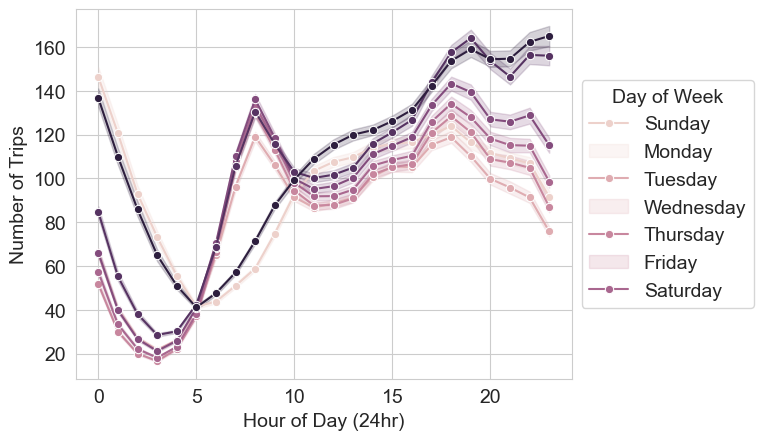
\includegraphics[width=0.5\textwidth]{plots/num_trips_day_time.png}%
}{%
  \caption{Average Demand by Hour and Weekday}%
}
\ffigbox{%
  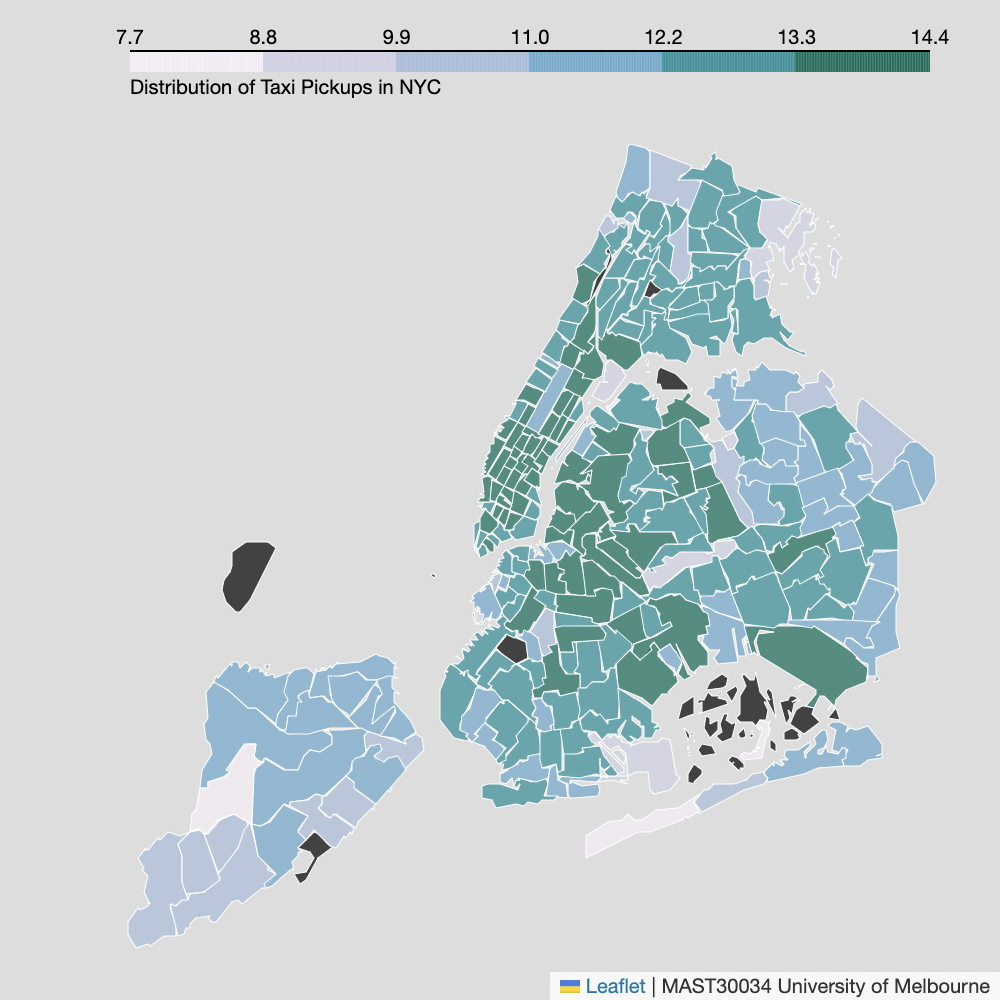
\includegraphics[width=0.5\textwidth]{maps/pickups.png}%
}{%
  \caption{Total Pickups (Log Scale)}%
}

\end{floatrow}
\end{figure}

\subsection{Pickup Zone}
The amount of pickups from different areas varies very heavily across the zones in New York, with very high density around popular areas like Central and Southern Manhattan, which are major business and tourism hubs (Figure 2). The demand is also extremely high in airports and major transportation hubs.

\subsection{Number of Businesses}
While the relationship between demand and the number of businesses in the area is complex at first, it becomes more apparent when we break it down by the borough. From Figure 3, we see a positive trend between the number of businesses in a zone and the demand, but the effect varies heavily by the borough. Yet, we see medium-high Pearson correlation values for all boroughs, indicating it may be a useful feature in our modelling when combined with the borough factor.

\begin{figure}[H]
\begin{floatrow}
\ffigbox{%
  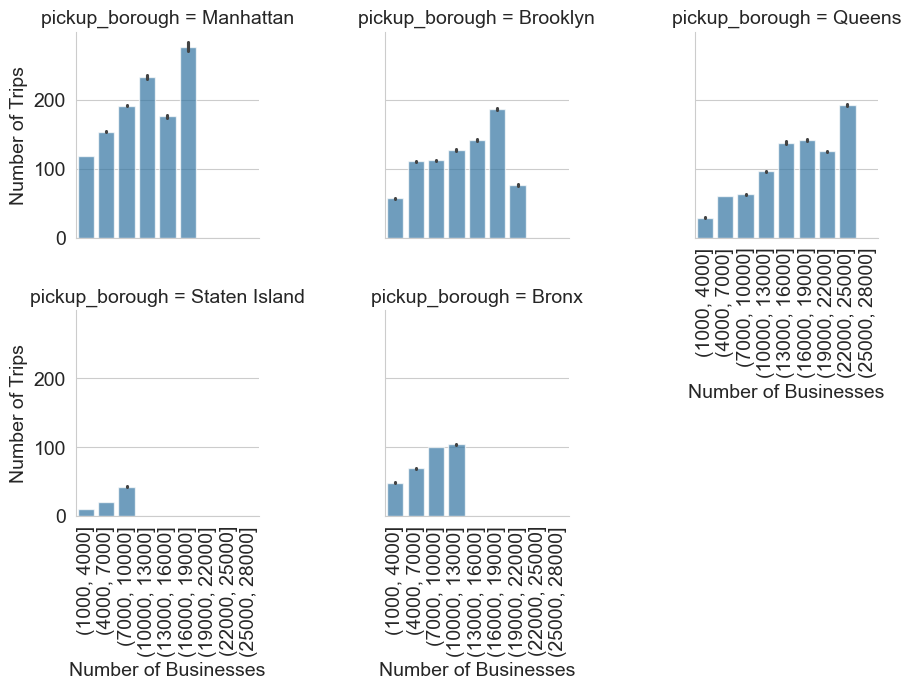
\includegraphics[width=0.5\textwidth]{plots/borough_trips.png}%
}{%
  \caption{Number of Businesses vs Number of Trips}%
}
\ffigbox{%
  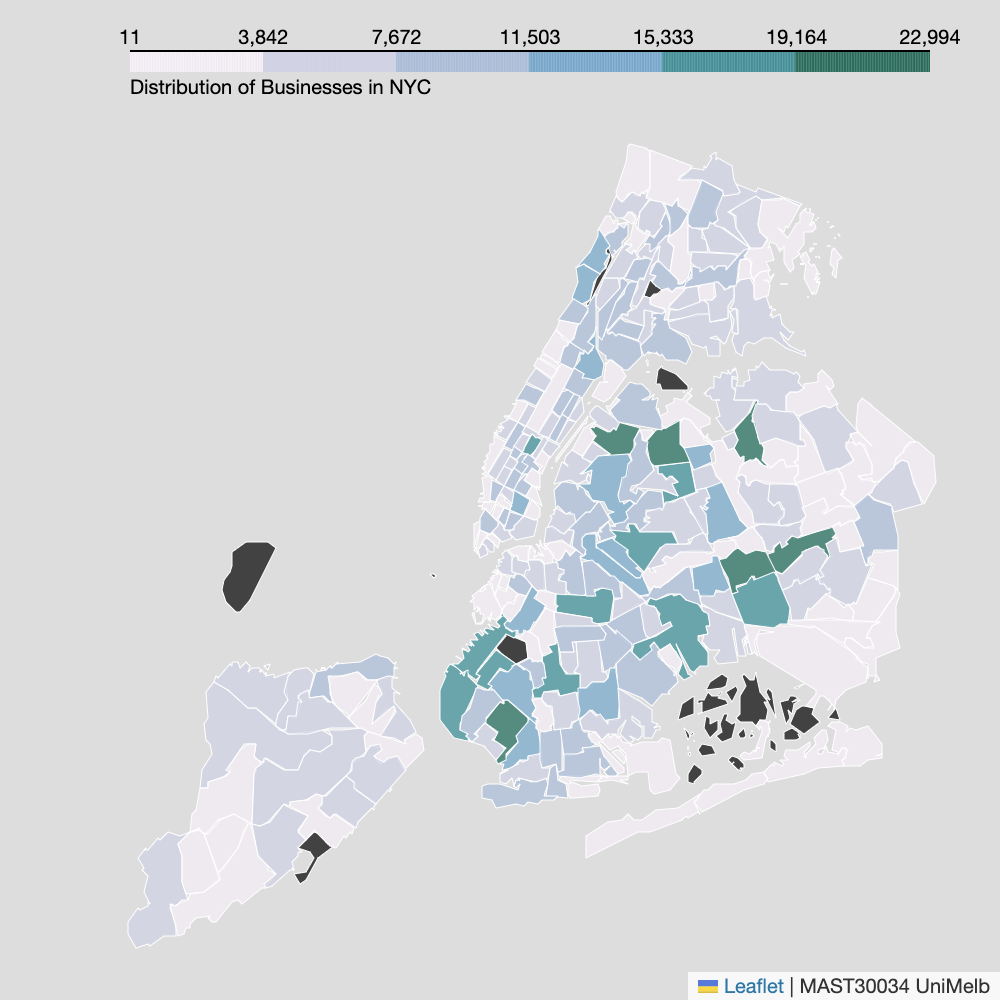
\includegraphics[width=0.5\textwidth]{maps/businesses.png}%
}{%
  \caption{Distribution of Businesses}%
}

\end{floatrow}
\end{figure}

\capbtabbox{%

\begin{tabular}{c c}
Borough & Pearson Correlation\\
\midrule
Bronx & 0.5784 \\
Brooklyn & 0.3681 \\
Manhattan & 0.4096 \\
Queens & 0.3016 \\
Staten Island & 0.4881 \\
\bottomrule
\end{tabular}
}{%
  \caption{Pearson Correlation between Number of Businesses in Area and Demand}%
}

\subsection{Inter-Borough Trips}
From Figure 11 (Appendix) we observe that most trips in NYC are within borough trips, with rare cross-borough trips. Most of these cross-borough trips start or end in Manhattan, hinting at the general importance of  Manhattan in NYC life. From previous research, NYC residents tend to live in the same borough as they work in and prefer public transport for long cross-borough travels\cite{communingpdf}. Further analysis may be done on the cross-borough trips and may be used by the Department of Transportation to optimise the public transport network.

\subsection{Surges}
Surges in demand are a critical opportunity for taxi providers to make use of unusually high demands. Usually, they may happen due to special events like concerts, parties or sports. Both companies can charge additional surge charges on these trips, and drivers concentrating around these in advance can heavily improve customer experience and even help organisers and planners ensure a smooth outflow\cite{uberpricing, lyftpricing}. In our analysis, we define a surge as an event when the demand is more than double the median demand in that area. From Figure 5, we see that surges are most common late at night from 1:00 AM to 4:00 AM, which from Figure 1, is usually a low-demand time. Drivers may tend to take breaks during those times and if they are correctly identified, we can encourage them to design their schedule around the surge for maximum profitability. Next, we analyse the surges by location using Figure 6 and observe that surges are much more common in some areas than others, especially around parks and event venues, further confirming our theory about special events driving surges.

\begin{figure}[H]
\begin{floatrow}
\ffigbox{%
  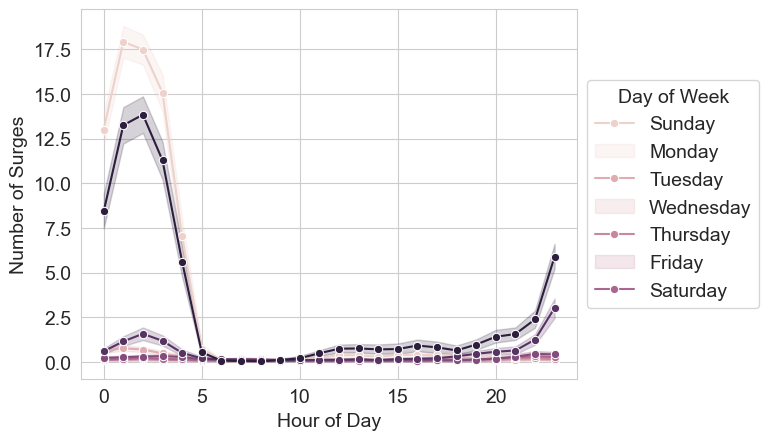
\includegraphics[width=0.5\textwidth]{plots/surges_plot.png}%
}{%
  \caption{Average Number of Surges by Hour and Day}%
}
\ffigbox{%
  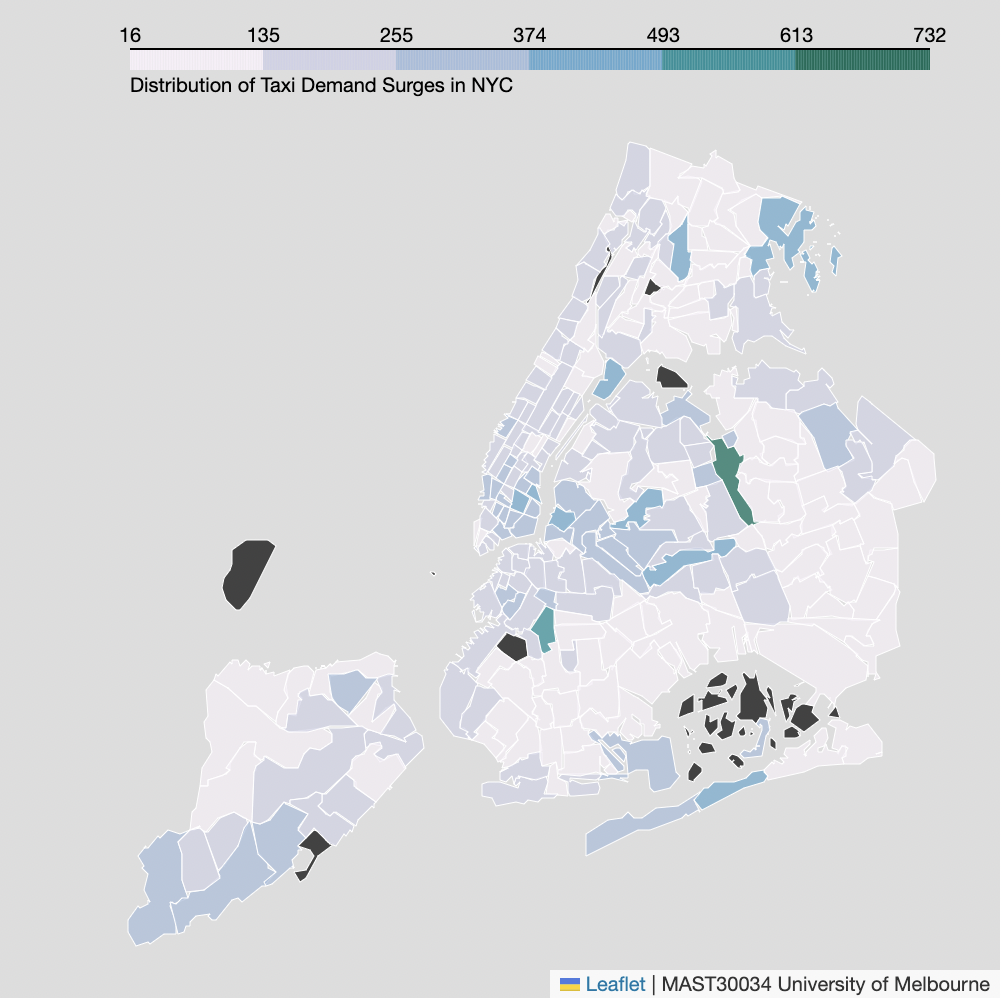
\includegraphics[width=0.5\textwidth]{maps/surges.png}%
}{%
  \caption{Locations with Most Frequent Surges}%
}
\end{floatrow}
\end{figure}

\section{Modelling}
\subsection{Chosen Factors}
To ensure the model is practically useful, we include readily available factors to model the demand in a particular location.
\begin{itemize} 
    \item Hour of Day and Day of Week (One-Hot Encoded)
    \item Number of Businesses in the respective zone
    \item Weather (Temperature, Relative Humidity, Rain, Snowfall, Wind Speed).
    \item Is Airport or not
    \item Borough (One-Hot Encoded)
    % use \item to create more points
\end{itemize}
\subsection{Assumptions}
This model makes some inherent assumptions, that should be considered while interpreting the output of these models, and in practical usage.
\begin{itemize} 
    \item We treat the hour of the day as a continuous variable, despite it being inherently cyclic in nature, to avoid feature space explosion and thus, over-fitting.
    \item We assume the size and distribution of businesses remain stable over time, and thus influence demand in predictable ways.
    \item Lastly, since zone-wise weather data is not available, we assume that the data collected at Central Park applies across New York and there aren’t major variations within the city. Further, we assume that future weather predictions are reasonably accurate for the practical usage of the model.
    % use \item to create more points
\end{itemize}
\subsection{Chosen Models}
Three Machine Learning models, namely Linear Regression (LR), Decision Tree Regressor (DTR) and XGBoost (XGB) were implemented to model the rideshare demand.

Firstly, Linear Regression (with L2 regularisation) was chosen due to its simplicity and interpretability. Since we standardise the data, we can look at the respective regression coefficients as an indicator of the relative importance of each feature.

Next, we move to some more complex models to gain a higher accuracy. App-based ride share businesses are known to not care about model interpretability over performance, and the loss of simplicity would be acceptable in most cases.

Since we have some important categorical predictors, we can use a Decision Tree Regressor to effectively model their impacts separately.

XGBoost, a widely recognized model for exceptional performance on tabular data, was included due to its superior performance in complex datasets\cite{xgboost}. It is an enhanced version of the Gradient Boosting Algorithm and includes L1 and L2 regularisation\cite{xgboost}.
\section{Discussion}
In this study, we chose Mean Absolute Error (MAE) as our performance metric. While Root Mean Squared Error (RMSE) is the metric used by training algorithms, we use MAE for practical inferences as it enables easier interpretation and comparison.

From Table 2, we see that while all models perform reasonably well, XGBoost significantly outperforms Linear Regression and Decision Trees in all boroughs, indicating a high complexity in the problem. With an error of ~36 rides in bustling areas like Manhattan with thousands of rides every hour, and even less for other boroughs, we see that our model is largely successful in modelling the complexity of taxi demands in New York, and is suitable for practical applications.

From Figure 7, we observe that Linear Regression and Decision Tree underfit on the pickup hour of day feature, which might be highly affecting their accuracy. Meanwhile, XGBoost is highly successful in modelling hourly fluctuations, with some bias towards underestimating the demand, which may be due to the generally increased demands in June, as per Figure 13 (Appendix). If this is the case, models trained on larger datasets spanning multiple years may be able to perform even better.
\begin{figure}[H]
\begin{floatrow}
\ffigbox{%
  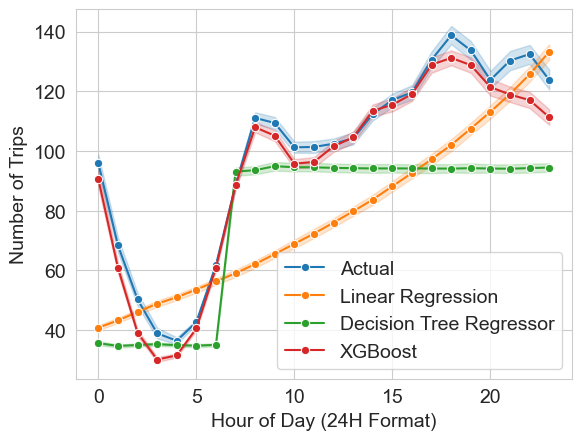
\includegraphics[width=0.5\textwidth]{plots/error_distribution_hour.png}%
}{%
  \caption{Errors on Test Data by Hour}%
}
\capbtabbox{%
\begin{tabular}{lccc}
\toprule
& & \textbf{MAE}\\
\textbf{Borough} & \textbf{LR} & \textbf{DTR} & \textbf{XGBoost} \\ \midrule
Bronx           & 26.87                      & 23.80                            & \textbf{11.55}   \\
Brooklyn        & 67.65                      & 55.99                            & \textbf{20.40}   \\ 
Manhattan       & 79.79                      & 68.44                            & \textbf{35.99}   \\ 
Queens          & 38.98                      & 35.09                            & \textbf{13.39}   \\ 
Staten Island   & 8.94                       & 9.31                             & \textbf{3.81}    \\ 
\bottomrule
\end{tabular}
}{%
  \caption{Performance of Models on Test Data}%
}
\end{floatrow}
\end{figure}

Lastly, we analyse the errors by location using Figures 8, 9 and 10, and we see that our models, especially XGBoost are highly reliable in most zones across NYC, but face trouble in some specific zones and airports. Notably, from Figure 2, the demand is much higher in these areas, and so even if the numeric error is high, the relative error is still very low.

\begin{figure}[H]
\begin{floatrow}
\ffigbox{%
  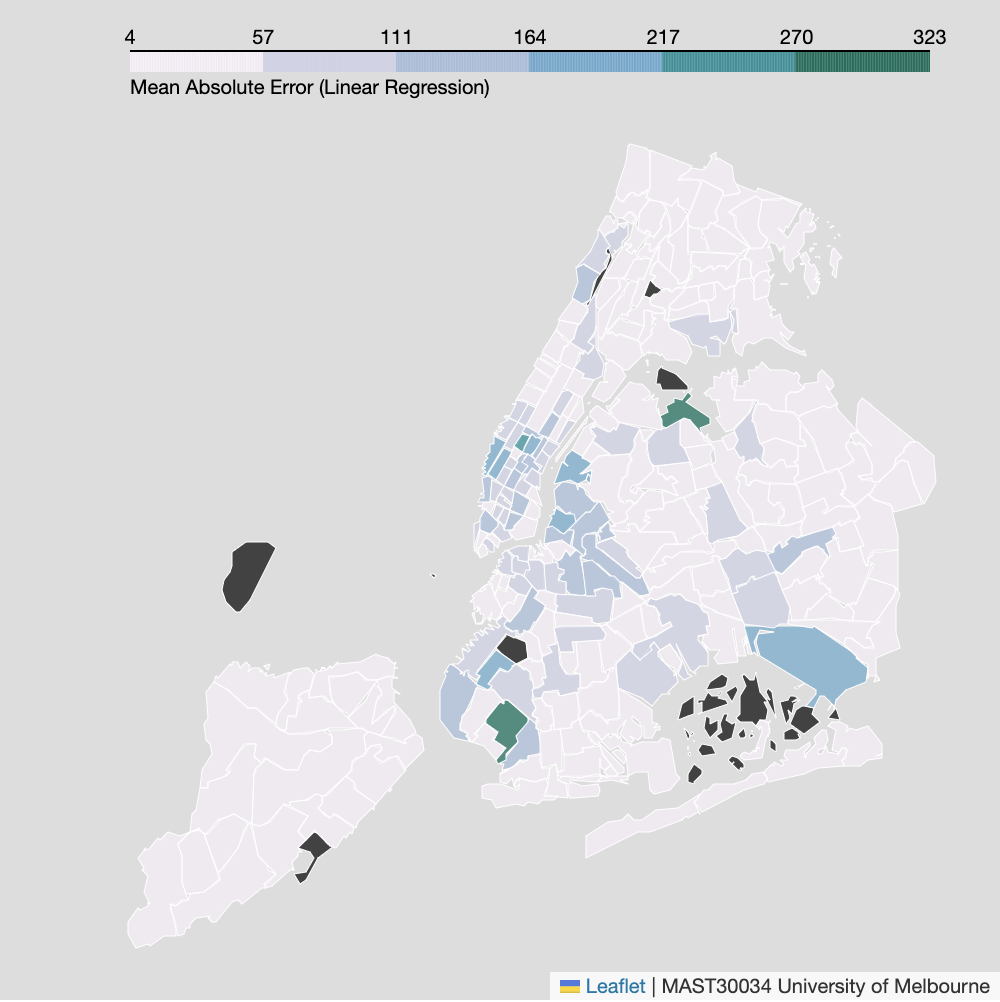
\includegraphics[width=0.5\textwidth]{maps/error_lr.png}%
}{%
  \caption{Linear Regression Errors}%
}
\ffigbox{%
  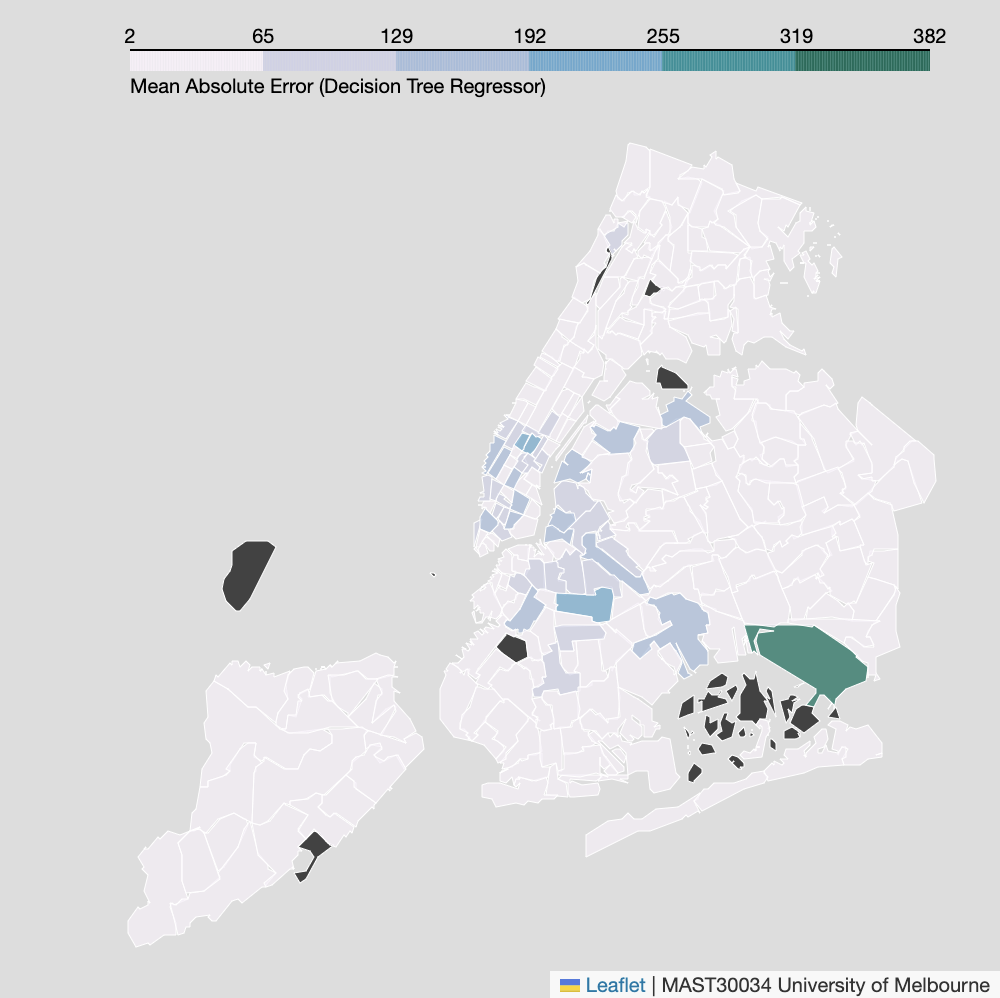
\includegraphics[width=0.5\textwidth]{maps/error_dtr.png}%
}{%
  \caption{Decision Tree Regressor Errors}%
}
\end{floatrow}
\end{figure}
\begin{figure}[H]
    \centering
    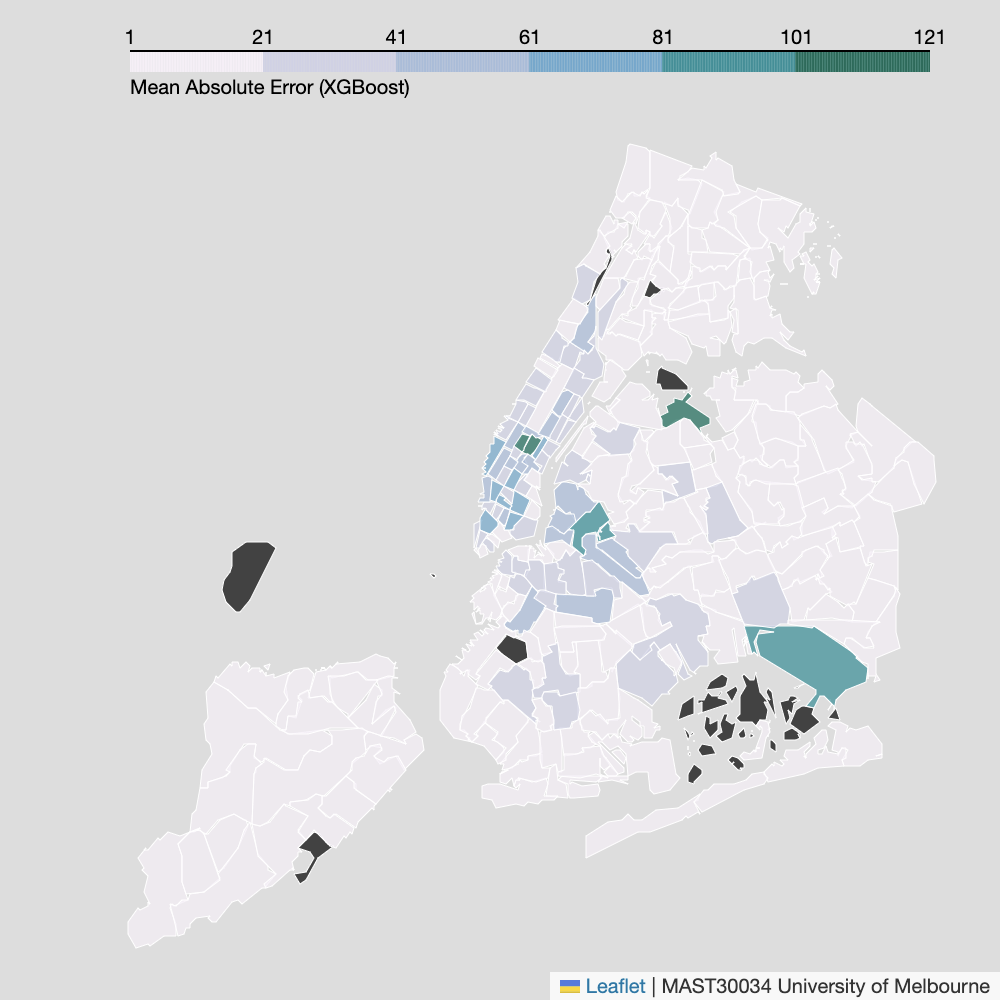
\includegraphics[width=0.5\linewidth]{maps/error_xgb.png}
    \caption{XGBoost Errors}
\end{figure}

\section{Recommendations}
As analysed above, the XGBoost model is very effective in modelling demand in most areas of New York. This can be used in real-time by ride-share companies to reorganise their fleet to meet the varying demand across the city. Their app-based nature allows them to send out notifications to divert drivers to high-demand locations and enhance user satisfaction and driver earnings. While this might increase cruising miles, the assurance that movements are made in the right direction helps negate their impact. Next, this can allow strategic management of driver rest times as companies can estimate the demand and allow excess drivers to rest. This can also help in electric car adoption as this makes strategic charge time scheduling possible. Lastly, these companies can invest in keeping a close eye on events in areas with high surge probabilities to predict them effectively and get the fleet prepared around those areas.

\section{Conclusion}
From our analysis, we see that the XGBoost model is highly effective at predicting the demand for most areas in NYC, especially with an overall mean of 95.63 and a very high standard deviation of 105.67 for the target variable. The external dataset of legally operating businesses helped us effectively model the demand by zone, which would have otherwise been a challenging task, as the amount of activity in different zones varies a lot across the city. In addition, the weather data helped us with the finer details of prediction.

For future improvements, companies may want to create separate models for airport demands as they might rely on airport flight schedules much more than the factors in current research. Next, the companies may develop overhead models that use these demand predictions to choose the best actions for individual drivers, optimising placement and rest times.


\clearpage

% BEGIN REFERENCES SECTION
\printbibliography
\clearpage
\section*{Appendix}
This section includes additional plots that weren't covered in the main analysis of the report but might be of further interest.
\begin{figure}[H]
    \centering
    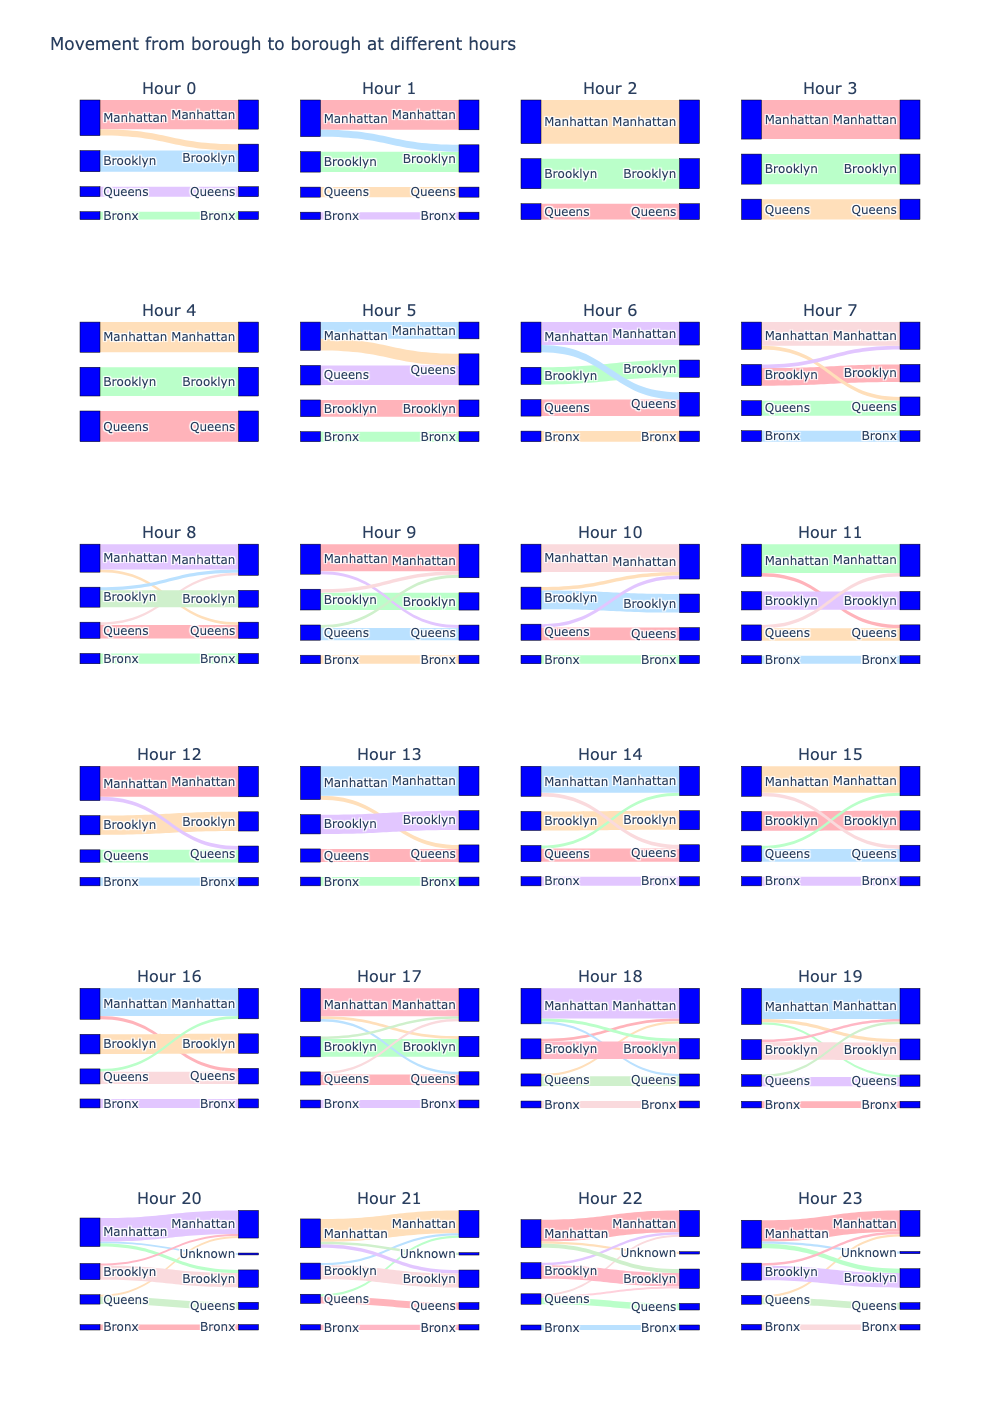
\includegraphics[width=0.7\linewidth]{plots/movement_plot.png}
    \caption{Cross borough movements in NYC, across the day}
\end{figure}
\begin{figure}[H]
    \centering
    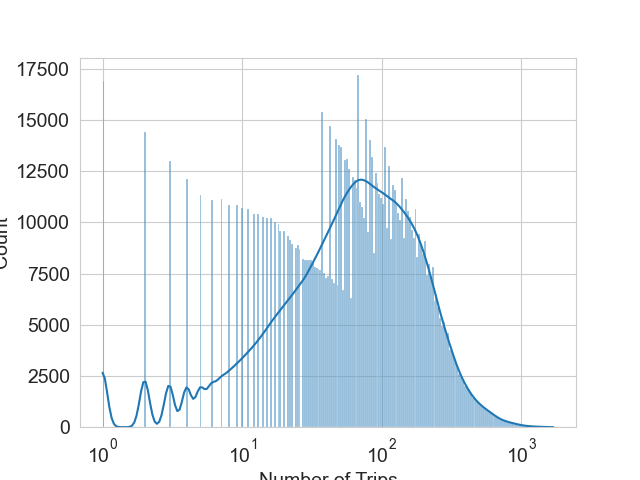
\includegraphics[width=0.7\linewidth]{plots/num_trips_distribution.png}
    \caption{Distribution of Label - Number of Trips in Zone per Hour}
\end{figure}
\begin{figure}[H]
    \centering
    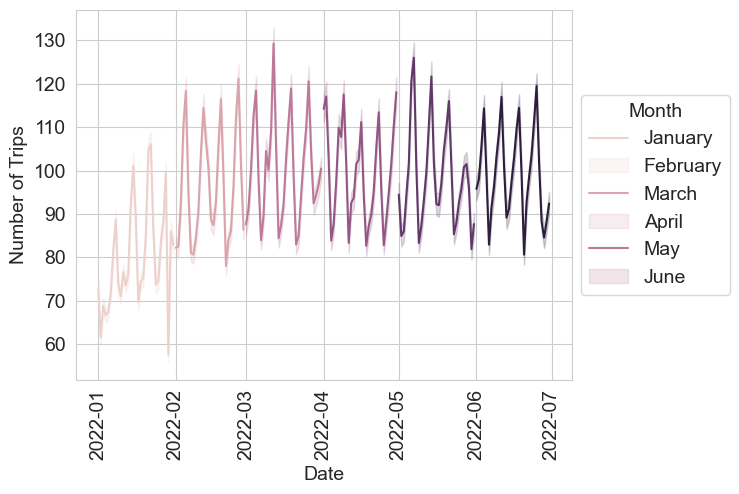
\includegraphics[width=0.7\linewidth]{plots/num_trips_monthly.png}
    \caption{Demand Timeline}
\end{figure}
\end{document}

